\documentclass{bioinfo}
\copyrightyear{2015} 
\pubyear{2015}

\access{ }
\appnotes{Manuscript Category}

\begin{document}
\firstpage{1}

\subtitle{Protein Classification}

\title[short Title]{Predicting Protein Subcellular Localization from Sequence Data}
\author[Sample \textit{et~al}.]{Eric Hambro\,$^{\text{\sfb 1,}*}$}
\address{$^{\text{\sf 1}}$eric.hambro.17@ucl.ac.uk, SN: 17096751, Machine Learning MSc, UCL }

\corresp{}%$^\ast$To whom correspondence should be addressed.}

\history{ }

\editor{ }

\abstract{\textbf{Motivation:}  
Predicting subcellular localization from raw sequence data is a important research problem, with applications in drug discovery and medecine research. 
This paper presents a comparison of two machine learning classifiers to do this: Random Forests and AdaBoost.
Using features derived from the sequence, these were trained to classify non homologuous protein sequences into four localizations: cytosolic, nuclear, secretory, mitochondrial.
These models were compared to each other and a baseline, and the best was chosen to predict localizations for X unknown proteins. \\
\textbf{Results:} The Random Forest classifier performed best in the comparison, with a test accuracy of 67.5\%, and F1 score of 68.3\% . This outperformed AdaBoost's 64.4\%  test accuracy and 62.6\% F1. Both beat the benchmark significantly, and the Random Forest model was chosen to make the final predictions.\\
% \textbf{Availability:} Text  Text Text Text Text
\textbf{Contact:} \href{eric.hambro.17@ucl.ac.uk}{eric.hambro.17@ucl.ac.uk}
}

\maketitle


%% TODO 
% * Introduction & fill in with experiments
% * Prediction of Proteins
% * Normalise CM
% * Error Bars on RocAuc
% * Refeences to pictures
% * Bagging Boosting Compare models
% * Conclusion
% * Abstract
\section{Introduction}

Discovering subcellular localization of proteins is a vital piece of information in many applied fields in cell biology. 
Not only is it important to help discover and catalogue the complex chemical pathways and signals that occur inside the cell, but it has vital medical applications, in particular in drug discovery and delivery. Furthermore, in cases where no homology is evident for a gene, subcellular localization of the protein can be used an indicator of the potential function of that protein - a vital clue in the right direction.

Since as early as \textbf{blah}, machine learning has been used to help predict automatically the subcellular localization of a protein, in an attempt to reduce the cost and time taken to process a protein sequences.  
Traditional methods of determining subcellular location, such as tagging proteins with immunofluorescence, were laborious and time intensive, and have been unable to keep up with the rapidly proliferating amount of genetic and protein sequence data. 
Using automated machine learning techniques, bioinformaticians have been able to make predictions at a high degree of confidence with only sequence data. One of the first of these models was \textit{cite and a sentence how it worked}, although today common methods include \textit{methods, cite 1}  and \textit{methods, cite 2}.

% Although sequence data of genes has proliferated since the advent of \textbf{technique}, the classification of protein function has lagged behind significantly.  \textbf{Statistic}. 
% This is partly down to the fact that protein function is a complex labelling task, given the function of proteins may vary under different conditions.  
% In cases where no homologues are present for a gene, knowing the subcellular location of the the protein gives indicator as to the proteins function. 
% Furthermore discovering subcellular location has proven to be vital information in the research of new drugs and vaccinations. 
% As such, automated means of predicting subcelular localization are utmost urgency in todays drug search enbironment.


In this particular experiment we are presented with a labeled data set of 9222 proteins and we will try to predict and evaluate both a Random Forests model and AdaBoost model on these data, comparing both to a baseline random model.
The proteins themselves each correspond to one of four subcellular localizations - cytosolic, secretory, nuclear or mitochondrial - and after training the models, we make predictions of locations for \textit{X} unknown proteins in these classes, before analysing our own test errors and models. 

Section 2 of this paper contains a brief background of biological and machine learning elements used in the experiment, whereas Sections 3 and 4 presents the methods and results of the experiments. In Section 5 a discussion of the results is presented, along with a comparison of the models, their features, and analysis of the errors. A short conclusion is presented in Section 6.

%Para 1: What is it & why is it important?
%Para 2: What are applications?
%Para 3: What is the history?

%In this analsysi we are presented with predicting 4 classes of locations: w, x, y, z. These are mutually exclusive categories, and our aim was to train a classifier to predict our things. 

%Section 2 of this report contains a description of the method, where section 3 presents the results. Section 4 presents a discussion of the results, breaking down the reasons for choosing the method, and providing analyses of the features, results and a comparison to another model. Finally, I present a comparison with existing work in the field and further work that could be done. 

 %is Often pro 
%Why is protein function hard to predict? What is protein location hard to predict? Why is it important?

\section{Background}

\subsection{Subcellular Localization \& Transport}

In eukaryotic cells, proteins are often highly adapted to fulfilling their specialist functions in the cell.
These functions can be very localized within organelles or other parts of the cell, and so the proteins are too adapted to the specific subcellular location in the cell. 
In order to faciliate transport of protein to its location, often a location signifier is in some way encoded into the structure of the protein.
This what's known as a target peptide (if heading to an organelle) or signal peptide (if secreted). 
These peptides can vary greatly in structure, depending on the final destination, and can be explored in greater depth in \cite{Alb00}. 
Sometimes they are removed by a signal peptidase, when they reach their destinations.
Below are some of the known features of signal and target peptides, as mentioned in the above book.

\begin{enumerate}
  \item {\textbf{Targeting Secretion}} 
%https://www.ncbi.nlm.nih.gov/books/NBK6322/

  Proteins headed toward secretory pathways often contain short amino acid encodings (say 16-30 amino acids long), occuring near the N-terminus of the protein. Often they include a domain or sequence that is particularly hydrophobic, and these hydrophobic residues may form an $\alpha$-helix. 

  \item {\textbf{Targeting Mitochondria}} 

  In the case of proteins headed to mitochondria, a \textit{mitochondrial targeting signal} of a peptide signal is often found at the N terminus of the protein. These often consist of alternating positively charged and hydrophobic amino acids, that come together to form an amphiphilic $\alpha$-helix. These this pattern (of positively charged residues on one side, and uncharged hydrophobic residues on another) is what is primarily recognised by the receptor proteins, rather than a specific sequence.

  \item {\textbf{Into The Nucleus}} 

  Proteins that require importing into the nucleus often contain a \textit{Nuclear Localization Signal}, which may consist of a sequence amino acids that are positively charged (often arginine and lysine) exposed on the surface of the protein. In contrast with the other target peptides, it appears these signals can occure almost anywhere in the chain, and often form loops. Many of these are still uncharacterised.  

   \item {\textbf{Out of the Nucleus (Into The Cytosol)}} 

  Proteins that are are being exported out of the nucleus and into the cytosol are often tagged with a \textit{Nuclear Export Signal}. 
  A known example of \textit{Nuclear Export Signal} consists of a chain of several (hydrophobic) leucines, interspersed with other amino acids, between them. 
  Since some proteins frequently move between the nucleus and the cytosol, it is common for some proteins to contain both  \textit{Nuclear Export Signals} and \textit{Nuclear Localization Signals}, which are effectively controlled by the cell to direct movement.



\end{enumerate} 


% In the case of a proteins headed toward secretion, these encodings are referred to as signal peptides. They are often 16-30 amino acids long, occuring near the N-terminus (the start) of the protein.In the case of a proteins headed toward secretion, these encodings are referred to as signal peptides. They are often 16-30 amino acids long, occuring near the N-terminus (the start) of the protein.
% These small peptides are called \textit{signal peptides}

\subsection{Bagging \& Boosting}
Our investigation compares two machine learning models to a benchmark random classifier, selecting the best. 
These two models (Random Forests and AdaBoost) were selected on account of being good are examples of common ensembling techniques: \textit{bagging} and \textit{boosting}.

\subsubsection{Bagging \& Random Forests}

Bootstrap aggregation (or \textit{bagging}) is an ensemble method to the reduce the variance of a prediction when using high variance classifiers. 
It involves, selecting many subsamples of the training data, and generating estimates from the average performance of classifiers trained on this data. 
Thanks to this averaging of predictions, overfitting our training data becomes less of a risk, since each classifier can overfit to it's subsection of the data without impacting the average too greatly in the end.

In a Random Forest, our high-variance classifier is a decision tree, and we adapt the \textit{bagging} algorithm to improve performance.
Specifically we only give each individual classifier access to a random subset of the features of the data, at training time.
The aim of this is to stop any correlation on the decision trees that may arise from their greedy behaviour, as they look through variables to select the best split point. 
By only having access to a random subset of features, the decision trees become less correlated, and the Random Forest algorithm produces a better 'averaged' estimate.

\subsubsection{Boosting \& AdaBoost}

The AdaBoost algorithm is a different method that uses a ensemble technique known as \textit{boosting}.
Instead of a combining votes from many high variance normal classifiers (like a decision tree), \textit{boosting} involves learning by combining lots of weak learners (like a decision stump), by training the on particularly chosen subsections of the data, and combining votes in a particular way. 
Specifically, each successive weak-learner is trained on selections of the data that aim to emphasise the most misclassified data points. 
These learners are then weighted by their error, to provide the overall classification.

%%% IF NEED PADDING: \textbf{In more detail, the algorithm goes as follows:}




\section{Method}

\begin{table}[!t]
\processtable{Experimental Data Set By Class\label{Tab:RawData}} {\begin{tabular}{@{}llll@{}}\toprule Cytosolic &Mitochondrial &Nucleic & Secreted  \\\midrule
3004 & 1299 & 3314 & 1605\\\botrule
\end{tabular}}{The total available labeled data used in this experiment.}
\end{table}

\subsection{Preprocessing}

Data was obtained from four files containing protein sequences in Fasta format. 
Each file contained proteins according to its type of subcellular localization: cytosolic, secreted, nuclear and mitochondrial. 
The number of proteins in each file is presented in Table \ref{Tab:RawData}. 
These data files contained no homologues, and therefore could be assimilated, shuffled and split into a training and validation set randomly. 
The data was then split into a test set that would be held out for final evalution (20\%), and a train and validation set (80\%) that could be used to tune hyperparameters. 
%\textbf{This was done, and a training-validation split of 70\%-30\% was set.}

The data was then fed through a pipeline to extract a number of features from the sequence.
These features all corresponded to floating point numbers, and so were concatenated to form a 75-dimensional feature vector, that would be used to train the models. 

\subsection{Features}

The open source `BioPython` module was used to extract features from the sequence data, allowing us to augment raw residue sequence data with important characteristics of the amino acids, such as isoelectronic point or molecular weight. 
In total 75 features were created, although many of these could be grouped into the same category. These features were:

\begin{itemize}


\item{ \textbf{Protein Length} } - An integer representing the length of the protein sequence, in residues.
\item{ \textbf{Amino Acid Composition} } - A float created for each amino acid, corresponding to the percentage composition of that amino amino acid in the protein.
\item{ \textbf{Aromaticity}} - A float corresponding to a measure of the aromaticity of the molecule according to Lobry et al\textit{1994}. This is measured by adding the frequencies of residues phenylalanine, tryptophan and tyrosine, in the sequence of the protein.
\item{ \textbf{Isoelectric Point}} - A float representing the isoelectric point of the protein according to values taken by Bjellqvist et al \textit{ref}.
\item{ \textbf{Molecular Weight}} - A float simply molecular weight of the protein. 
\item{ \textbf{Secondary Structure Features}} - Three separate features were created indicating the fraction of amino acids which tend to be either $\alpha$-helixes, $\beta$-sheets, or turns/loops. These amino acids were: $\alpha$ - Val, Ile, Tyr, Phe, Trp, Leu;   $\beta$ - Glu, Met, Ala, Leu; \textit{loops} -  Asn, Pro, Gly, Ser
\item{ \textbf{Start/End Amino Acid Composition} - Two floats were created for each amino acid, according to the percentage composition of that amino amino acid in the first and last 20 residues of the protein respectively.}

\end{itemize}

These features were chosen as they had a high impact on the on the remaining the accuracy of the classifier. 
The importance of each of these features to various classifications is examined in section 4.  


\subsection{Classifier Training \& Tuning}

Three classifiers were trained to investigate the best possible model in predicting the subcellular location. These models were:

\begin{itemize}
  \item {Categorical Distribution Classifier (Benchmark)}
  \item {Random Forests Classifier}
  \item {Adaboost Classifier}
\end{itemize}

All classifiers were implemented using the open source `scikit-learn` package. In all cases, model parameters were fit with a 5-fold cross validation, on the train and validate set mentioned previously. 
Hyperparameters were tuned using a grid search, and chosing the parameters that had the best 5-fold cross validation score of accuracy. 
The best of these 5-fold models was then taken for each classifier, and was tested on the held out test set, evaluating both the overall accuracy, and the precision and recall of individual categories.

It is worth noting that in the Random Forests Model, multiple models were trained, each solely to predict one class, instead of a single multi-class classifier. 
Although this is strictly unnecesssary for a Random Forests Classifier, it provides the additional advantage of allowing for interpretable feature importances, and more interpretable analysis of the individual class classifiers. 
To ensure a fair analysis of the classifier, a single multi-class Random Forests Model was also implemented, though this was found to have the same accuracy as the individual models, to within experimental error.
In this multi-model case, `scikit-learn' provided the best means for creating the 4 mutually exclusive classifiers from Random Forests, using it's One-Vs-Rest Classifier wrapper.

\subsection{Benchmarks}

A raw, bottom level benchmark for this investigation was a random classifier, here referred to as the Categorical Classifier. 
This classifer is so called because it simply predicted categories for data points following a simple categorical distribution, with the probability vector $\mathbf{p}$ learnt from the calculating frequency of each class in it's training set.
This model was implemented by hand, using the inheritance properties of `scikit-learns' BaseEstimator class, to allow easy integration into the scikit-learn pipeline.

% $$x \sim Categorical(\mathbf{p}) \text{ where } \mathbf{p} = [0.25, 0.25, 0.25, 0.25]$$

% \subsection{Ablation Study \& Feature Evaluation }
% To investigate and evaluate the performance of certain features, an ablation study was performed on the each of the above categories.
% An ablation study was performed, by removing one feature at a time and testing the 5-fold cross validation score of the model in predicting these data. 
% The results are presented \textit{fig xyz}

\section{Results}

\subsection{Final Hyperparameters}
Table \ref{Tab:hyperp} shows results of the hyperparameter grid search for each of the models, presenting the best hyperparameters according to the mean cross-validation accuracy. These hyperparameters were the ones used for all following data analysis.

\begin{table}[!h]
\processtable{Hyperparameters of Model\label{Tab:hyperp}} {\begin{tabular}{@{}lll@{}}\toprule Model  & Hyperparameter & Settings \\\midrule
Categorical (Benchmark) & N.A. &  N.A.   \\
% Logistic Regression & param1 & row1 \\
% Logistic Regression & param2 & row1 \\
% Random Forests Classifier (MC) & estimators & 450 \\
Random Forests Classifier & estimators & $450$ \\
Adaboost Classifier & estimators & $200$ \\
                    & learning rate & $0.25$ \\\botrule
\end{tabular}}{}
\end{table}

% \begin{table}[!h]
% \processtable{Hyperparameters of Model\label{Tab:hyperp}} {\begin{tabular}{@{}lll@{}}\toprule Model  & Hyperparameter & Settings \\\midrule
% Categorical & N.A. &  N.A.   \\
% Logistic Regression & param1 & row1 \\
% Logistic Regression & param2 & row1 \\
% Random Forests Classifier (MC) & estimators & 450 \\
% Random Forests Classifier (OvM)& estimators & 450 \\
% Adaboost Classifier & estimators & $300$ \\
% Adaboost Classifier & learning_rate & $0.25$ \\\botrule
% \end{tabular}}{}
% \end{table}


\subsection{Model Scores}
With the hyperparameters selected and 5-fold cross-validation performed, the most accurate models from the cross-validation were chosen as "final models", and evaluated on the held out test data-set. 
Table \ref{Tab:acc} shows both the results of the cross-validation accuracy (both train and validation), and the accuracy and F1 score of the best model on the held out test set.
Further interrogation of these models in then presented in Table \ref{Tab:metr}, where the precision, recall and F1 score of each of the classes for each model is presented.

\begin{table}[!h]
\processtable{Accuracy of Models\label{Tab:acc}} {\begin{tabular}{@{}lllll@{}}\toprule Model  & CV Train Acc & CV Valid Acc  & Test Acc & Test F1 \\\midrule
Categorical (Benchmark) & $0.283 \pm 0.004$ & $0.291 \pm 0.011$ & $0.277$ & $0.273$ \\
% Random Forests Classifier (MC) & y &  Test Acc &row2 \\
Random Forests  &  $1.00 \pm 0.000$  &  $0.682 \pm 0.005$ & $0.675$ & $0.683$\\
AdaBoost  & $0.650 \pm 0.003$ & $0.634 \pm 0.013$ & $0.643$ & $0.626$\\\botrule
\end{tabular}}{}
\end{table}

\begin{table}[!h]
\processtable{Classification Metrics\label{Tab:metr}} {\begin{tabular}{@{}llllll@{}}\toprule  Model & Class & Precision  & Accuracy & F1 & Support\\\midrule
Categorical  & Cyto & $0.326$ & $0.333$ & $0.329$ & $604$ \\
        & Mito & $0.144$ & $0.140$ & $0.142$ & $271$ \\
        & Nucl & $0.363$ & $0.363$ & $0.363$ & $653$ \\
        & Secr & $0.210$ & $0.206$ & $0.208$ & $316$ \\
\midrule
Random Forests & Cyto & $0.602$ & $0.556$ & $0.578$ & $604$ \\
        & Mito & $0.804$ & $0.668$ & $0.730$ & $271$ \\
        & Nucl & $0.639$ & $0.714$ & $0.674$ & $653$ \\
        & Secr & $0.837$ & $0.880$ & $0.858$ & $316$ \\
\midrule
AdaBoost & Cyto & $0.506$ & $0.495$ & $0.500$ & $604$ \\
        & Mito & $0.694$ & $0.661$ & $0.677$ & $271$ \\
        & Nucl & $0.589$ & $0.640$ & $0.613$ & $653$ \\
        & Secr & $0.895$ & $0.807$ & $0.849$ & $316$ \\\botrule

\end{tabular}}{Metrics calculated on test set, using best trained model}
\end{table}

From these tables it is clear that not only did the Random Forests Model perform best overall but it also performed best in every single individual class. AdaBoost performed only slightly worse in accuracy, $0.643$ compared to Random Forests $0.675$, although it performed worse under the F1 metric ($0.626$ compared to $0.683$), where the F1 metric was an average of class F1s, weighted by the number of classes present in the test set. Both models significantly outperformed the categorical benchmark, with its accuracy of $0.277$.

Furthermore in all cases, the test set accuracies were very close to the mean cross-validation accuracies, which themselves had low variance. This indicates little overfitting of the hyperparameter choice to the validation set - as desired.

\subsection{Predictions}

Since the Random Forest Model was selected as our best model, it was subsequently used to to make predictions of \textbf{YYY} hitherto unclassified proteins. These prediction, along with percentage confidence scores, are given in Table \ref{Tab:predict}.

\begin{table}[!h]
\processtable{Predictions of Test Proteins\label{Tab:predict}} {\begin{tabular}{@{}lll|lll@{}}\toprule Protein ID  &  Location & Probabilty & Protein ID  &  Location & Probabilty\\\midrule
SEQ677 & Cyto & 0.416  & SEQ608 & Cyto & 0.472  \\
SEQ231 & Cyto & 0.307  & SEQ402 & Mito & 0.628  \\
SEQ871 & Nucleus & 0.381  & SEQ433 & Secreted & 0.804  \\
SEQ388 & Cyto & 0.360  & SEQ821 & Secreted & 0.795  \\
SEQ122 & Cyto & 0.430  & SEQ322 & Nucleus & 0.680  \\
SEQ758 & Nucleus & 0.560  & SEQ982 & Nucleus & 0.813  \\
SEQ333 & Cyto & 0.494  & SEQ951 & Nucleus & 0.483  \\
SEQ937 & Cyto & 0.686  & SEQ173 & Cyto & 0.495  \\
SEQ351 & Cyto & 0.517  & SEQ862 & Mito & 0.662  \\
SEQ202 & Mito & 0.694  & SEQ224 & Cyto & 0.381  \\\botrule
\end{tabular}}{Predictions made with Random Forest model}
\end{table}


\subsection{Plots}

Finally, to investigate the importance of various features, the ROC curves were plotted for our Random Forests model  (Figure \ref{fig:roc}), along with the confusion matrix for its classifications (Figure \ref{fig:confusion}). 
Furthermore the top 25 importance weights of the individual classifiers were also plotted, to aid in this investigation. 
These are presented in Figures \ref{fig:import1} \&  \ref{fig:import2} .

% A final model was produced that was able to achieve a classification score of 68.2\%.  The returning operator characteristic (ROC) curves were plotted for each predictor in the class and are shown in table \textit{blah}. The confusion matrix was also plotted for the test set, indicating where classifications were errornious. Finally the predictions for the unknown test scores are presented in table {XYZ}.


\section{Discussion}

\subsection{Classifier Comparison}

It is unsurprising that that both boosting and bagging methods far outperformed the benchmark method. 
The woeful performance of $0.277$ accuracy is to be expected for a model that doesn't take into account any of the sequence data, or underlying features. 
However, the significant discrepancy between Random Forests and AdaBoost is more difficult to explain, and probably comes down to the high variance nature of the underlying data. 
In general, boosting methods struggle on very noisy data, as in the best cases bagging acts to reduce variance, whereas bagging tends to reduce bias. 
It is interesting to note that the AdaBoost classifier only really approached Random Forest performance in the case of the Secreted label (RF $0.858$ vs Ada $0.849$), which is probably the class with the least `noise', or strongest `signal', judging by the strength of the leading feature importances.

\begin{figure}[!h]
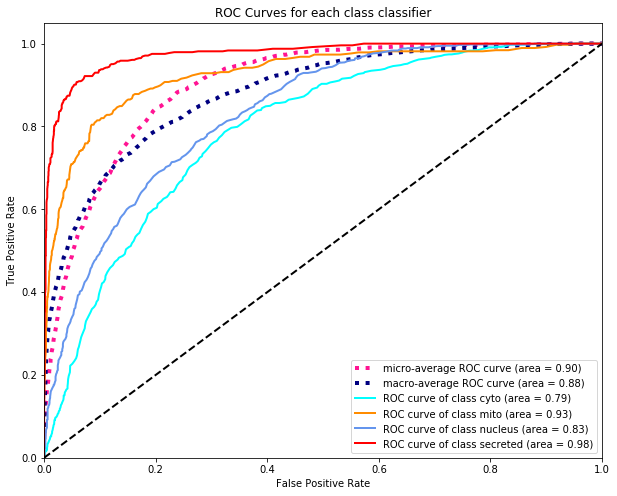
\includegraphics[width=8cm]{roc_curve}
\caption{Returning Operator Characteristic (ROC) curves for each classifier in Random Forests }
\label{fig:roc}
\centering
\end{figure}

This performance difference is likely down to the difficulty that \textit{boosting} methods have in dealing with high variance datasets.. 
\begin{figure}[!h]
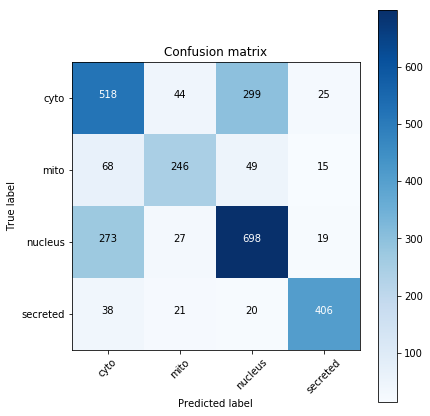
\includegraphics[width=8cm]{confusion}
\caption{Confusion Matrix for Random Forest Classifier}
\label{fig:confusion}
\centering
\end{figure}

\begin{figure}[t]
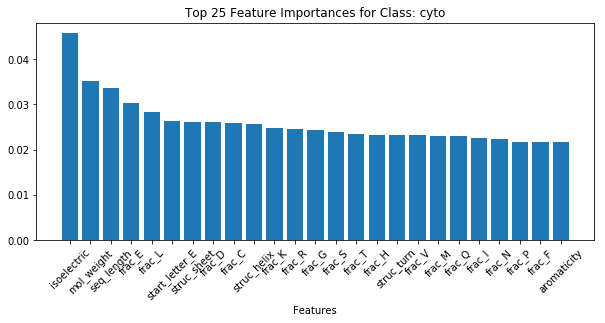
\includegraphics[width=8cm]{cyto_import}
\centering
% \end{figure}\begin{figure}[h]
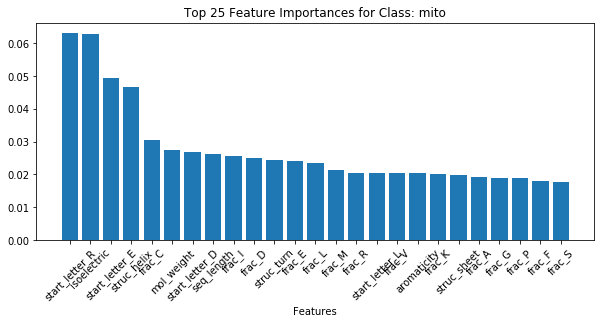
\includegraphics[width=8cm]{mito_import}
\centering
% \end{figure}\begin{figure}[h]
\caption{Top 25 Feature Importances for Cytosol and Mitochondrial classes in Random Forests Classifier}
\label{fig:import1}
\end{figure}



Although both the feature-based models performed to different levels on the test set, it is striking that both models found the same classifications difficult. 
Both models' F1 scores for classes run from lowest to highest in the same order: cytosolic, nuclear, mitochondrial, secreted.
This seems to suggest an underlying challenge with distinguishing these former classes, either due to true biological similarity, or simply lack of features.

This is also supported by examining the confusion matrix for the Random Forests classifier (Figure \ref{fig:confusion}).
It appears that the greatest single sources of error come from misclassifying nuclear labels for cytosolic ones, and vice versa. Almost $25\%$ of nuclear proteins are misclassified as cytosolic, and $36\%$ as cytosolic as nuclear.

This misclassification is made all the more evident by looking at the Returning Order Characteristic (ROC) curves, where all the classifiers are plotted together. 
From these graphs, it is immediately clear that the best classifier is the secreted class, with the area under curve (AUC) of 0.98, followed by the mitochondrial class of 0.93. The worst performer is the cytosolic class (0.80) followed by the nuclear class (0.84), as also visible from the curves.

From a biological perspective, there are also a number of reasons why it is conceivable that these particular protein classifiers (cytosolic and nuclear) should perform worse than the other two categories (secreted and mitochondrial). 
For one thing, since a number of proteins frequently move between the nucleus and the cytosol, it is possible that many proteins may may posses both \textit{Nuclear Export Signals} and \textit{Nuclear Localization Signals}. 
This mixup of very distinct features (in the form of target peptides) would likely lead the classifiers to struggle to distinguish the correct class in ambiguous cases.

Furthermore, it is likely that mitochondrial proteins and secreted proteins may have important macroscopic properties (aside from target peptides) that still show up in our choice of features.
For instance There may exist restrictions on mitochondrial proteins, that need to be perhaps a certain size or make up, help in the respiration process.

% At any rate it is clear from the ROC curves in particular that secretion is particularly well detected, with nuclear and cytoplasmic classes are easier to confuse. An analysis of the exact features that could be responsible for this are presented in the next section.


% As mentioned previously, peptides destined for a certain subcellular location often have sequences of peptides encoding this. It is likely these are strong features in this sequence analysis, and will be examined in the netx Furthermore, it is likely that peptides operating in a certain part of the cell might have specific features, related to it specific function

% The strength of the secreted and mitochondrial classes i two classes as classifiers is at least partly down to the very specific nature of proteins these locations. For a protein to be secreted, there is a requirement that it is able to be transported across the cell membrane, and this puts some restrictions on the form the protein can take. \textbf{what restriction}. Similarly the mitochondrial proteins are highly likely to be used in respiration in some respect and so are likely again to have features that indicate this. 
% However, there are many proteins that are frequently transported between the nucleus and the cytosol, meaning that it can be hard to distinguish these proteins from features.
% A more specific look at the features, and what they can be used to discern, is examined in the following section.

\begin{figure}[t]
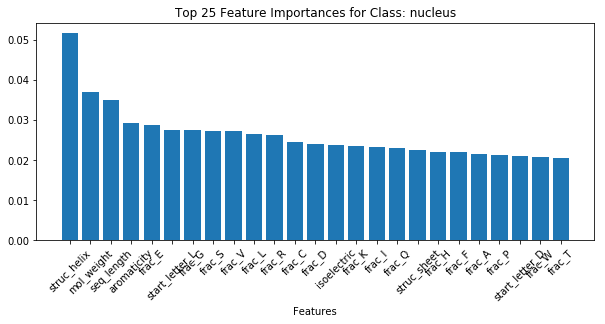
\includegraphics[width=8cm]{nucleus_import}
\centering
% \end{figure}\begin{figure}[h]
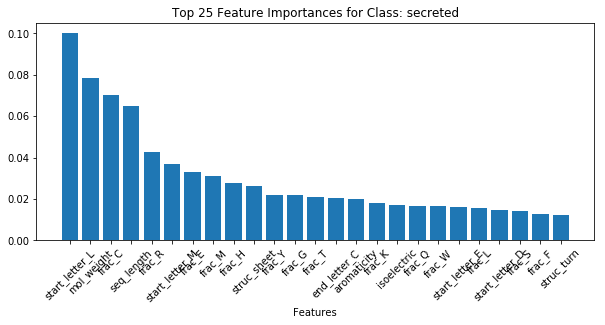
\includegraphics[width=8cm]{secreted_import}
\caption{Top 25 Feature Importances for Nucleus and Secreted classes in Random Forests Classifier}
\label{fig:import2}
\centering
\end{figure}
\subsection{Error Analysis}

\subsection{Features Analysis}

Perhaps more interesting than the comparison of the two different models is the close comparison of the features that have had a significant impact on the model.
By inspecting Random Forest Model's feature importances, we have a natural way of interpreting the significance of each features to each classifier.

The first thing to notice is the relative scales of the four graphs, in comparison to one another. The secreted classifier (Fig \ref{fig:import2}) has a much stronger set of "significant" features, than all the other classes. 
In the case of comparison to nucleus and cytoplasmic classes, secreted's top feature is over twice the importance of the latter classes' highest feature. 
Furthermore its top 4 features features all have higher importances than the highest single feature for these classes.  
This indicates that there are distinct `killer features' for this class, which explains why both AdaBoost and Random Forests scored particularly highly on this class.
From the importances, it appears these features are highly tied to the fraction of Leucines and Cysteines at the start of the sequence, and the molecular weight and sequence length.

Next to notice is that, as mentioned in the initial background, mitochondrial proteins also have importances of features matching the description of the \textit{mitochondrial targeting signals}. 
These target peptides sometimes consist of alternating positively charged and hydrophobic amino acids forming a helix, so correspondingly our strongest features include features noting isoelectricity, structural helices, and the presence of positively charged Arginine at the start of the sequences.

When it comes to nuclear and cytosolic proteins, it's worth noting that the second and third best importance features - molecular weight and sequence length - are shared. 
This indicates some of the difficulty these classes have in distinguishing themselves.  
Furthermore these features are broad macroscopic features that do not really indicate a particular target sequence, also making it harder to classify these proteins. 
In fact, even the "strongest feature" for each of these classes is a macroscropic feature - isoelectric point, and helix fraction - indicating our set of features haven't been able to pick up the nuclear target peptides.

It is finally worth noting that none of the most important features correspond to peptides at the end of the sequence, only the start.  This is fairly good evidence that something important happens at the N-terminus of a protein, and supports background theory that this is where target peptides are often found.


\subsection{Further Improvements}

Although this model performed well in distinguishing the secreted and mitochondrial proteins there are a number of additional features that may particularly improve future implementations of this model. 

First, some measure of hydrophobicity would be a valuable additional feature. 
As mentioned in section 2, often the hydrophobic characteristic of signal peptides is what is detected by receptors, but this model only captures these features indirectly, through looking at frequencies of individual amino acids.
A specific feature for hydrophobicity wasn't added due to the lack of there being an available hydrophobicity scale in the BioPython module, but it is likely some measure of this (both over the whole molucule and just the N terminus), would be of some value.

Secondly, it might be worth exploring and searching for specific target patterns within the model. 
When exploring potential features, I attempted to search for these by creating a feature for all possible "bigrams" and "trigrams" of residues, and examining importances after training, but the high dimensionality made learning difficult and slow. 
Instead, if one had specific examples of known target peptides this feature would likely greatly help classification, without adding too much to computational complexity.
A drawback would be that these examples may be very incomplete, as many signals are still unknown, so there may be a limited benefit.

Finally it may be worth exploring the use of neural networks, as classifiers.
Neural networks have shown significant promise in various fields in bioinformatics including protein function prediction \textbf{Jones et al}, and could theoretically be applied to this problem. 
In this case, one could use a richer set of features and feed through a multiclass deep neural network, or even augment the sequence data with features and the feed augmented sequence into recurrent neural network, such as an LSTM. 
This latter architecture might have the advantage of allowing investigators to detect new target peptides, through spotting sequences that radically increase likelihoods of a certain classification.
However, a draw back is that these neural methods often require a great deal of data, and the dataset here is relatively small so a neural model may not generalise well.
This method should be considered, if more training sequence is avaliable.

\section{Conclusions}

In conclusion, it was clear that the Random Forests algorithm performed best when predicting the subcellular locations of proteins, achieving an F1 score of 0.683, and accuracy of 0.675. This beat the AdaBoost classifier, with F1 of 0.626 and accuracy of 0.643, although both models far surpassed a random benchmark based on a categorical distribution, with its F1 of 0.273 and accuracy 0.277. 

The outperformance of the Random Forests algorithm, compared to AdaBoost, is likely due to the very noisy data that occurs in this field, and performance only really started to become comparable, when `killer features' were present for a class. However, both models seemed to struggle with same class classifications, which indicated an underlying difficulty with biological features, rather than the algorithms themselves.

In particular, cytosolic and nuclear proteins were easily mixed up, likely due to the fact that both \textit{Nuclear Export Signals} and \textit{Nuclear Localization Signals} can be present on the same protein, and also are not restricted to only appearing at the N-terminus, making them harder to pick out. 
Secreted and mitochondrial class classifiers performed much better, and had feature importances that supported the current biological understanding of signal peptides such as \textit{mitochondrial targeting signals}, and their structure. 

Finally I concluded that the above experiment, while carried out well (with a hold out test accuracy performing very similarly to the cross-validation accuracy), could be improved by the addition of a number of extra features, including hydrophobicity or counting of known target peptide subsequences. Also in the case of being presented with more labelled data, I suggest neural methods could be used to tackle this problem with some success. 





\vspace*{-10pt}


% \section*{Acknowledgements}


%\bibliographystyle{natbib}
%\bibliographystyle{achemnat}
%\bibliographystyle{plainnat}
%\bibliographystyle{abbrv}
%\bibliographystyle{bioinformatics}
%
%\bibliographystyle{plain}
%
%\bibliography{Document}


\begin{thebibliography}{}

\bibitem[Alberts, \textit{et~al}. (2008)]{Alb00}
Alberts, \textit{et~al}. (2008) Molecular Biology of the Cell
(5th ed.), \textit{Book Title}, 2nd edn. Publisher, Location, Vol. 1, pp.
???--???.



\bibitem[Bofelli {\it et~al}., 2000]{Boffelli03}
Bofelli,F., Name2, Name3 (2003) Article title, {\it Journal Name}, {\bf 199}, 133-154.

\bibitem[Bag {\it et~al}., 2001]{Bag01}
Bag,M., Name2, Name3 (2001) Article title, {\it Journal Name}, {\bf 99}, 33-54.

\bibitem[Yoo \textit{et~al}., 2003]{Yoo03}
Yoo,M.S. \textit{et~al}. (2003) Oxidative stress regulated genes
in nigral dopaminergic neurnol cell: correlation with the known
pathology in Parkinson's disease. \textit{Brain Res. Mol. Brain
Res.}, \textbf{110}(Suppl. 1), 76--84.

\bibitem[Lehmann, 1986]{Leh86}
Lehmann,E.L. (1986) Chapter title. \textit{Book Title}. Vol.~1, 2nd edn. Springer-Verlag, New York.

\bibitem[Crenshaw and Jones, 2003]{Cre03}
Crenshaw, B.,III, and Jones, W.B.,Jr (2003) The future of clinical
cancer management: one tumor, one chip. \textit{Bioinformatics},
doi:10.1093/bioinformatics/btn000.

\bibitem[Alberts, \textit{et~al}. (2000)]{Aut00}
Auhtor,A.B. \textit{et~al}. (2000) Chapter title. In Smith, A.C.
(ed.), \textit{Book Title}, 2nd edn. Publisher, Location, Vol. 1, pp.
???--???.

\bibitem[Bardet, 1920]{Bar20}
Bardet, G. (1920) Sur un syndrome d'obesite infantile avec
polydactylie et retinite pigmentaire (contribution a l'etude des
formes cliniques de l'obesite hypophysaire). PhD Thesis, name of
institution, Paris, France.

\end{thebibliography}
\end{document}
